\documentclass{beamer}
\usepackage[utf8]{inputenc}
\usepackage{graphicx}
\usepackage{tikz}
\usepackage{appendixnumberbeamer}

% Thème minimal
\usetheme{default}
\usecolortheme{dove} % gris clair

% Pied de page avec bandeau de couleur
\definecolor{mygray}{RGB}{50,50,50} % gris foncé pour le bandeau

\setbeamertemplate{footline}{%
  \leavevmode%
  \begin{beamercolorbox}[wd=\paperwidth,ht=2.5ex,dp=1ex,leftskip=1em,rightskip=1em,center]{footlinecolor}
    \color{white}Raphaël ADDI, Mehdi DHAHRI – INSA Toulouse
    \hfill
    \insertframenumber/\inserttotalframenumber
  \end{beamercolorbox}%
}
\setbeamercolor{footlinecolor}{bg=mygray, fg=white}
\setbeamertemplate{navigation symbols}{} % Supprimer les icônes inutiles

% Informations générales
\title{Modélisation de la parole par LPC}
\author{Raphaël ADDI, Mehdi DHAHRI}
\institute{INSA Toulouse – Département 3MIC}
\date{17 avril 2025}

\begin{document}

% Slide 1 – Titre
\begin{frame}
  \titlepage
\end{frame}

% Slide 2 – Modélisation LPC
\begin{frame}{Modélisation LPC de la parole}
  \begin{itemize}
    \item Objectif : modéliser le signal vocal via un filtre AR.
    \item \( x[n] = \sum_{k=1}^{p} a_k x[n-k] + e[n] \)
    \item Excitation :
    \begin{itemize}
        \item bruit blanc : sons non voisés
        \item train d’impulsions : sons voisés
    \end{itemize}
  \end{itemize}
\end{frame}

% Slide 3 – Analyse et Synthèse
\begin{frame}{Analyse et Synthèse LPC}
  \begin{itemize}
    \item \textbf{Analyse LPC} :
    \begin{itemize}
        \item Découpage en trames, fenêtrage Hann
        \item Estimation des coefficients via moindres carrés
        \item Mesure d’erreur (normes L1 et L2)
    \end{itemize}
    \item \textbf{Synthèse LPC} :
    \begin{itemize}
        \item Reconstruction du signal à partir d’une excitation
        \item Synthèse croisée : transfert spectral entre deux voix
    \end{itemize}
  \end{itemize}
\end{frame}

% Slide 4 – Reconnaissance vocale
\begin{frame}{Vers la reconnaissance vocale}
  \begin{itemize}
    \item Extraction des formants (fréquences et amplitudes)
  \end{itemize}

  \centering
  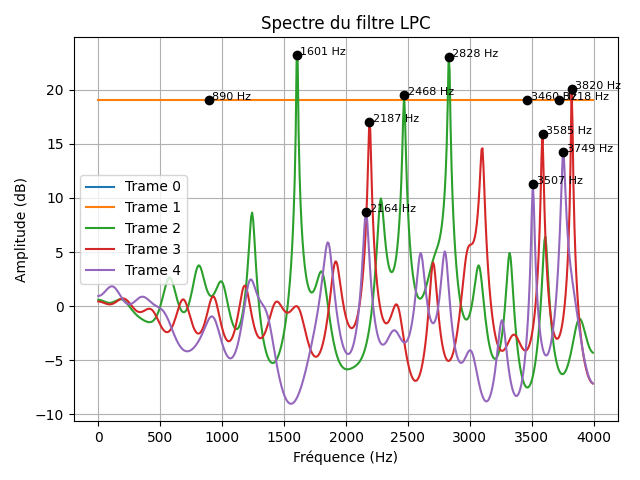
\includegraphics[width=0.6\linewidth]{Spectre_du_filtre_LPC_formants_speech_french.png}
  
  \vspace{0.1em}
  {\tiny Figure : Spectre du filtre LPC avec formants annotés (en Hz)}

  \vspace{0.8em}
  \begin{itemize}
    \item Comparaison aux formants d’un dictionnaire \texttt{.wav}
    \item Fonction \texttt{EstimationSon(...)} : détermine le son le plus proche
    \item Correction temporelle avec \texttt{CorrectionSon(...)}
  \end{itemize}
\end{frame}




% Slide 5 – Conclusion
\begin{frame}{Conclusion et perspectives}
  \begin{itemize}
    \item LPC = compression, synthèse, transformation
    \item Application directe à la reconnaissance vocale basique
    \item Perspectives :
    \begin{itemize}
        \item robustesse au bruit
        \item meilleure excitation vocale
        \item reconnaissance multi-locuteur
    \end{itemize}
  \end{itemize}
\end{frame}

\end{document}
